\begin{figure}[htbp]
    \centering
    \resizebox{\linewidth}{!}{%
    \begin{tikzpicture}[
        font=\sffamily,
        box/.style={
            draw,
            thick,
            align=center,
            inner xsep=12pt,
            inner ysep=16pt,
            text width=4.8cm,
            minimum height=3.6cm
        },
        side/.style={
            align=center,
            text width=4.0cm
        },
        arrow/.style={-{Stealth[scale=1.2]}, thick},
        biarrow/.style={{Stealth[scale=1.2]}-{Stealth[scale=1.2]}, thick},
        lbl/.style={align=center, font=\large\bfseries},
        edgeLbl/.style={font=\small, midway, fill=white, inner sep=2pt}
    ]

    % 1. Bloque de la App Móvil (Extremo Izquierdo)
    \node[side] (movilGroup) at (0,0) {
        \begin{tikzpicture}[scale=0.8]
            \draw[thick, rounded corners=3pt] (-0.35, -0.6) rectangle (0.35, 0.7);
            \draw[fill=black] (0, -0.45) circle (1.5pt);
            \draw[thick] (-0.15, 0.45) -- (0.15, 0.45);
        \end{tikzpicture} \\[6pt]
        \large \textbf{App Móvil}\\
        \vspace{4pt}
        \normalsize Captura de audio crudo del usuario y envío de fragmentos.
    };
    \node[lbl, above=0.6cm of movilGroup] (movilTitle) {Captura};

    % 2. Bloque del Gateway (A la derecha de la App)
    \node[side, right=1.6cm of movilGroup] (gatewayGroup) {
        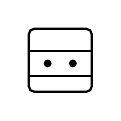
\begin{tikzpicture}[scale=0.8]
            \draw[thick, rounded corners=2pt] (-0.5, -0.5) rectangle (0.5, 0.5);
            \draw[thick] (-0.5, 0.15) -- (0.5, 0.15);
            \draw[thick] (-0.5, -0.25) -- (0.5, -0.25);
            \draw[fill=black] (-0.2, -0.05) circle (1.5pt);
            \draw[fill=black] (0.2, -0.05) circle (1.5pt);
        \end{tikzpicture} \\[6pt]
        \large \textbf{Gateway}\\
        \vspace{4pt}
        \normalsize Control de estado y búfer de sesión.
    };
    \node[lbl, above=0.6cm of gatewayGroup] (gatewayTitle) {Orquestación};

    % 3. Bloque de Procesamiento Lingüístico
    \node[side, right=1.6cm of gatewayGroup] (aiGroup) {
        
\begin{tikzpicture}[scale=0.8]
            \draw[thick] (0,0) circle (0.3cm);
            \foreach \a in {0,60,120,180,240,300} {
                \draw[thick] (\a:0.3cm) -- (\a:0.45cm);
            }
        \end{tikzpicture} \\[6pt]
        \large \textbf{Procesamiento\\Lingüístico e IA}\\
        \vspace{4pt}
        \normalsize \englishText{ASR} (Whisper), \englishText{PLN} (NER Médico)
    };
    \node[lbl, above=0.6cm of aiGroup] (aiTitle) {Inteligencia Artificial};

    % 4. Bloque de Estándares (A la derecha del Procesamiento)
    \node[side, right=1.6cm of aiGroup] (stdGroup) {
        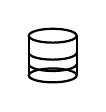
\begin{tikzpicture}[scale=0.8]
            \draw[thick] (0,0.35) ellipse (0.38 and 0.11);
            \draw[thick] (-0.38,0.35) -- (-0.38,-0.28);
            \draw[thick] (0.38,0.35) -- (0.38,-0.28);
            \draw[thick] (0,-0.28) ellipse (0.38 and 0.11);
            \draw[thick] (-0.38,0.08) arc (180:360:0.38 and 0.11);
            \draw[thick] (-0.38,-0.1) arc (180:360:0.38 and 0.11);
        \end{tikzpicture} \\[6pt]
        \large \textbf{Normalización\\Clínica}\\
        \vspace{4pt}
        \normalsize Codificación en SNOMED CT / CIE-10.
    };
    \node[lbl, above=0.6cm of stdGroup] (stdTitle) {Capa de Estándares};

    % 5. Generación de Informes Médicos 
    \node[side, below=1.2cm of aiGroup, xshift=2.8cm] (informesGroup) {
        
\begin{tikzpicture}[scale=0.8]
            \draw[thick] (-0.4,-0.5) rectangle (0.4,0.5);
            \draw[thick] (-0.2,0.2) -- (0.2,0.2);
            \draw[thick] (-0.2,-0.1) -- (0.2,-0.1);
            \draw[thick] (-0.2,-0.3) -- (0.1,-0.3);
        \end{tikzpicture} \\[6pt]
        \large \textbf{Generación de\\Informes Médicos}\\
        \vspace{4pt}
        \normalsize Generación de informes médicos con LLM y exportación a FHIR.
    };

    % Conexiones secuenciales principales
    \draw[arrow] (movilGroup.east) -- node[edgeLbl, above] {\englishText{WebSocket}} (gatewayGroup.west);
    \draw[biarrow] (gatewayGroup.east) -- node[edgeLbl, above] {\englishText{Por cada chunk}} (aiGroup.west);
    \draw[biarrow] (aiGroup.east) -- (stdGroup.west);
    
    % Conexión corregida hacia informes medicos: 
    \draw[arrow] (gatewayGroup.south) -- ++(0,0) |- node[edgeLbl, above] {Al finalizar la sesión} (informesGroup.west);

    \end{tikzpicture}%
    }
    \caption{Diagrama arquitectónico horizontal detallando el flujo de datos y la separación de entidades.}
    \label{fig:diagrama_arquitectura_horizontal}
\end{figure}